% Physics of membrane and related stuff

\section[Neuronal operation]{Neuronal operation\label{sec:Physics-MembranesChannels}\label{sec:Physics-Components}}

%\section{Neuronal components}

In this section, we discuss statical and dynamical
components, attribute a new role to the 
\gls{AIS}, and introduce the \hyperlink{DynamicLayer}{dynamic layers} on the surfaces of the membrane.
Fundamentally, only electrical and thermodynamic forces exert on ions,
but the biological environment decisively affect their movement.
As discussed in section~\ref{sec:Physics-Thermodynamics}, in biological systems, a complex set of forces exerts on ions, see Eq.(\ref{eq:NernstPlanckExtended}). 
We derived the "thermodynamic electrical field" in section~\ref{sec:Physics-ElectrolyteThermalField}, so we use the
concept of "thermoelectric field" to describe the exerting forces.
Considering the forces, 
orients us to discover the phenomena and their reasons. 
As discussed in section~\ref{sec:Calculating-ion's-speed}, 
the ions move with their Stokes-Einstein speed, proportional with
the generalized electrical field, see Eq.(\ref{eq:StokesCurrent}),
so enormously different speeds form the neuronal operation.
Furthermore, because of their cooperation, it is hard to separate the 
operation of the components.

The dynamic components do not fit in the 'old understanding'.
Physiology inherited the static view of anatomy and developed
its own static methods of observation (clamping, see section~\ref{sec:PHYSICS_clamping}), as discussed at several 
points of the site. That concept has no place for dynamically
formed components (a consequence of the finite neuron size and ion speeds).
Recall that, in physics, the \href{https://en.wikipedia.org/wiki/Drift_velocity}{drift speed} and the \href{https://en.wikipedia.org/wiki/Thermal_velocity}{thermal speed} differ by several orders of magnitude; furthermore, that they describe the same object's macroscopic and microscopic movement
However, they are interpreted for a system of neutral particles; the ions
behave differently. We also introduce the electrical \gls{potential-assisted speed}
(scales to between the drift speed and thermal speed)
and the \gls{potential-accelerated speed} (scales to well above the thermal speed) of
ions that differ by  several orders of magnitude.
Of course, these speeds have no well-defined values,
but they orient us in discussing the ions' behavior.
Speed plays a decisive role in biology~\cite{RoleOfInformationTransferSpeed:2022}.


\subsection[Animal electricity]{Animal electricity\label{sec:PHYSICS_ANIMALELECTRICITY}}

%\begin{advanced}
\quotationbox{
“All animals that move have electricity in their bodies.
Electricity is the only thing that’s fast enough to carry the messages
that make us who we are. Our thoughts, our ability to move,
see, dream, all of that is fundamentally driven and organized by
electrical pulses. It’s almost like what happens in a computer but
far more beautiful and complicated.”
--(neuroscientist Rodolfo Llinas quoted in “Electricity’s spark
of life” by Emily Sohn in Science News for Students, 29
September 2003).
}
%\end{advanced}

(We note that the communication, of course, can be seen as electrical pulses
when studied by discipline 'electricity' and can be seen as
mechanical pulses (solitons) when sudied by another discipline.
The speed of biological electricity is million times slower
that the speed of electromagnetic pulses, and matches speed of
the sound in biological fluid. 
The waves of the fluid show electrical behavior because 
the waved medium contains also ions.)

The phenomenon that the body operates with electric signals was discovered about one and a half century ago~\cite{HelmoltzHistory:1851},
and the idea that "In simple cases of ionized substances both the amount of
substance and the force acting may be expressed in electrical terms"~\cite{COLE_CURTIS_IMPEDANCE:1939} shined up nearly a century ago. 
The basic idea of \hypertarget{BiologicalCurrent}{biological current} was correctly defined at the beginning:
"The permeability of a membrane to a penetrating substance is
given quantitatively by the amount of the substance which crosses
a unit area of the membrane in unit time under the action of a unit
force. In simple cases of ionized substances both the amount of
substance and the force acting may be expressed in electrical terms.
Then the permeability may be ultimately converted into coulombs
per second for a square centimeter and a potential difference of 1
volt, which is the conductance, in reciprocal ohms, for a square
centimeter"~\cite{COLE_CURTIS_IMPEDANCE:1939}.
However, at that time physiologically defined fine details were not known.
\index{conductance}
\index{current!biological}
One must never forget that "\textit{movement of
ions} across the plasma membrane \textit{results in changes of electrical potential}
across the membrane, and these potential changes are the primary signals
that convey biological messages"~\cite{JohnstonWuNeurophysiology:1995}
(\textit{using "\indexit{equivalent electrical circuit}s" hides that the potential changes}).
In this section, we proceed along the line pointed by those latter authors in Chapter 2 of their book. 

We must recall that \textit{this charge is delivered chemically,
i.e., it is the result of an thermoelectric process}, so the concentration and the potential change simultanously.
Also, \textit{the charge carriers are ions instead of electrons and the transfer mechanisms are entirely different}.
From purely simplistic considerations concerning the  many orders of magnitude in the ratio of their size and mass, we see that the charge carriers have speeds differing by orders of magnitude, that requires revisiting the classic laws such as instant interaction (behind the ideas such as Kirchoff's laws, Ohm's law, 'retarded potential').
Furthermore, the ions are not fixed to isolating surfaces, and some biological "constructions" may be active elements from the point of view of electronics: the membrane may store charge  (disappears) for some period and ion channels may "produce" charge in the measured system.
Also, the molecules may dissociate and polarize under the effects of local potentials, enabling to create macroscopically different parameters such as potential and concentration, see also \hyperlink{Onsager_relations}
{Onsager's reciprocal relations}~\cite{OnsagerExperimental:1959}. 
In the case of living matter, we must handle thermodynamical and electrical forces simultanously. The are no 'net abstract' cases
where only electrical forces act on the ions. This feature, accompanied by the slowness and large size of the ions, requires attention and rethinking the basic notions of electricity.

We must also call attention to the dynamic behavior of charges
inside living matter. Basically, they are balanced, but, and it is vital for describing the life, they can get unbalanced in a local region for shorter or longer periods. This balanced state is the basis for having a resting potential (longer), and the perturbed (unbalanced) state is the basis for creating and transferring action potential, among others. \textit{The change of those states are described by the laws of motion, and their continuous change is the life itself.}

Although it is fundamentally correct that "because dissociated ions carry electric charges, their movement is influenced not only by concentration gradients but also by electric fields", these gradients are competing with each other and their complex interaction controls the biological processes. "Based on thermodynamic principles,
ions tend to flow from regions of high concentrations to regions of low
concentrations" (see~\cite{JohnstonWuNeurophysiology:1995}, page 9), furthermore, the electric gradient gets more role than presumed; see \hyperlink{Onsager_relations}
{Onsager's reciprocal relations}~\cite{OnsagerExperimental:1959}. 
We must never forget that \textit{ions represent both charge and mass,
so a current means delivering mass and vice versa}.
%
In some cases, when precisely measuring the time course of current
compared to the time course of voltage, one can experience a 'phase delay'
between them. This may inspire further research, such as inventing
'inductive', 'capacitive' and 'resistive' currents in electricity; or one may believe
that the system shows 'non-ohmic' behavior in biology; that is, it cannot be described
by laws of physics.

An often forgotten thought is that
"The things that neurophysiologists typically want to measure
are electrical signals such as action potentials and synaptic potentials,
or the membrane currents responsible for these potentials. \textit{Under ideal
circumstances, the physical act of measuring a neurophysiological event
would have no effect on the electrical signal of interest. Unfortunately,
this is seldom the case in neurophysiology.}"~\cite{JohnstonWuNeurophysiology:1995}, Appendix A. We do not want to repeat the content of that appendix, except some
points where we add notes, corrections or pinpointings.
We add, however, that neurophysiologists make measurements in
hybrid circuits, where the charge carriers are ions in one half of the circuit and electrons in the other. The conversion introduces several issues, among others delays (resulting 
in measuring non-matching value  pairs); introducing negatively
charged high-speed particles into systems having positively charged low-speed particles; intermixing inhomogenous, non-isotropic, structured matter into the systems and applying laws
derived for homogeneous, isotropic, unstructured matter; applying laws derived for the "free electron cloud" to the case of slowly moving dipole molecules.

It is worth to recall: "\textbf{Accuracy}: The degree to which a measurement indicates the true magnitude of a measurable quantity. \textbf{Precision}: The resolution and reproducibility of a measurement; implies nothing about accuracy. A measurement can be precise without being accurate. The reverse, however, is usually not true."~\cite{JohnstonWuNeurophysiology:1995} We add: sometimes, we measure a quantity which differs from the one we wanted to measure. Especially, if we interpret erronously what we wanted to measure and how do we measure it. That is exacly the case when the model is wrong.


\subsection{Ion channels and pumps\label{sec:Physics-IonChannels}\label{sec:Physics-ResourcesIonChannels}}

"The function of \hypertarget{Ion_Channel}{ion channels} is to allow specific inorganic ions
to diffuse rapidly down their electrochemical gradients across the lipid bilayer...
\index{lipid!bilayer}
Nerve cells (neurons), in particular, have made a specialty of using ion channels,
and ... use a diversity of such channels for receiving, conducting, and transmitting signals...
\textit{Ion channels cannot be coupled to an energy source to perform active transport,
so the transport that they mediate is always passive ('downhill')}" \cite{MolecularBiology:2002}.
(We note that the 'downhill' transport requires moving
the ions in a viscous fluid against friction, so it requires energy.
Due to the finite resources, discussed in section~\ref{sec:Physics-Resources}, the moved charge changes its potential energy to kinetic
energy plus dissipation. That potential energy (the membrane's potential) is the source to perform a 'passive' transport, given that the ion affects the membrane's field; for details see section~\ref{sec:Physics-BackgroundLogistics}.
The 'passive transport' would defy energy conservation.) 

The role of ion pumps must be revisited, too. According to
biology,
the ion channels and ion pumps have different charge transmission mechanism.
"These pumps differ from ion channels in two
important details. First, whereas open ion channels
have a continuous water-filled pathway through which
ions flow unimpeded from one side of the membrane
to the other, each time a pump moves an ion, or a group
of a few ions, across the membrane, it must undergo a
series of conformational changes. As a result, the rate of
ion flow through pumps is 100 to 100,000 times slower
than through channels. Second, pumps that maintain
ion gradients use energy, often in the form of adenosine triphosphate (ATP), to transport ions against their
electrical and chemical gradients. Such ion movements
are termed active transport."~\cite{PrinciplesNeuralScience:2013}, page 101.
\index{ion transport}
The so called "Na-K pump" \textit{is supposed} to actively transport (using energy from \gls{ATP})
sodium ions out of the cell and potassium ions into the cell.
However, in the old model no mechanism is provided how the ions gain energy from \gls{ATP} and how the ions are moved (what are the \textit{laws of motion} of ions in those ion channels and what a force (see Eq.(\ref{eq:IonicForces0}) 
can "transport ions against their electrical and chemical gradients").
Instead, some magic
mechanism by protein conformations \textit{is supposed}
without explaining what is the driving force to do so,
how it can deliver the ions in
sufficiently short times needed for the operation,
ans what is the source of the energy needed to move 
the huge amounts of molecular masses,
needed for implementing .


%\subsubsection{Ion channels}


We want to describe the change of voltage due to
limited resources using an idea similar to the predator-prey model.
We have charged sheets (represented by ions in the electrolyte) with potential $U_H$ and $U_L$
on the two surfaces of the membrane, 
plus we consider 
the corresponding neighboring layers on their side toward the "bulk" of the segment. We assume that the layers'capacity is constant, so the change of charge is linearly proportional to the change of the voltage.


\begin{figure}
\iflatexml
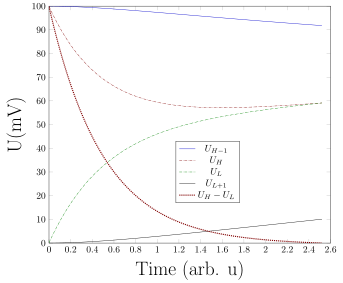
\includegraphics[width=0.65\textwidth]{fig/IonChannelRK.svg}
\else
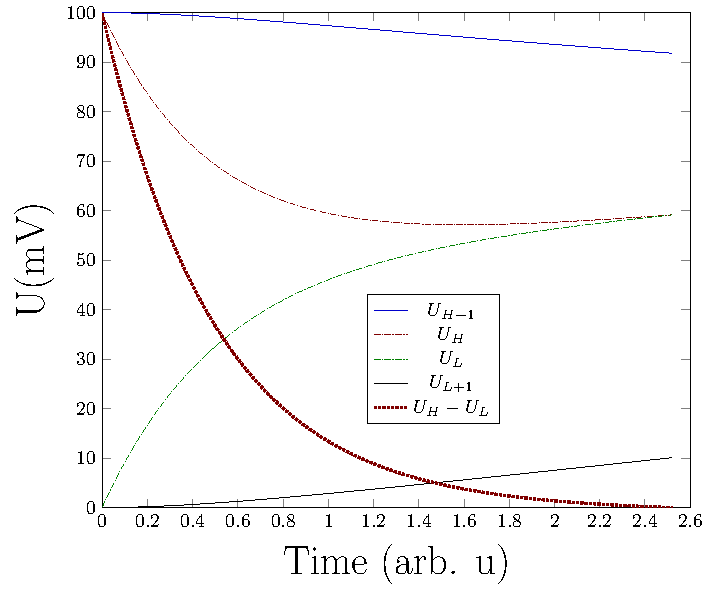
\includegraphics[width=0.65\textwidth]{fig/IonChannelRK.pdf}
\fi
	
	\caption{The potential values connected to the operation of ion channels. The arbitrary values of the transfer speeds (for visibility instead of approach real values) are $\alpha = 1$; 
	$\beta  =.1$; $\gamma = 0.0001$; furthermore the time scale is also arbitrary.
	\label{fig:IonChannelRK} }	
\end{figure}



We consider that a charge transfer happens from the layer with potential~$U_H$~to the layer with potential~$U_L$~
(that is, the \textit{same charge} is removed and added, respectively) with a high speed (we call it \textit{potential-accelerated} speed),
\index{potential-accelerated speed}
 furthermore, that with a much lower speed 
(we call it \textit{potential-assisted} speed)
\index{potential-assisted speed}
the charge in the neighboring layer increases and decreases, respectively, those voltages are ($U_{H-1}$~and~$U_{L+1}$). 


That is, we assume four voltages and the initial conditions
\[
U_{H-1} = U_{H} = U; \quad U_{L=1} = U_{L+1} = 0;
\]
%	
We assume a constant capacity for the layers and that the amount of transferred charge (or voltage) is proportional to the difference of voltages in the respective layers.
\[
\frac{dU_{H}}{dt} =  -\alpha * (U_H-U_L) + \beta *(U_{H-1}-U_H)
\]
%
\[
\frac{dU_{L}}{dt} = +\alpha * (U_H-U_L) - \beta *(U_{L}-U_{L+1})
\]
%
Furthermore, we assume that the after-diffusion from and to the layers next to the proximal layers is much lower than the high speed of the charge exchange
between the proximal layers, that is
\[
\frac{dU_{H-1}}{dt} = -\gamma*(U_{H-1}-U_{H})
\]
%
\[
\frac{dU_{L+1}}{dt} = +\gamma*(U_{L}-U_{L+1})
\]

As Fig.\ref{fig:IonChannelRK} depicts, voltages $U_H$ and $U_L$
quickly approach their balanced values. When they get equal, the driving force cancels.
In the meantime, the voltages $U_{H-1}$ and $U_{L+1}$ tend to approach $U_H$ and $U_L$, respectively.
 The diffusional and energy producing processes, depending on the local conditions, change the voltages
on the two ends of the channel, creating the illusion that the channel opens and closes. As~\cite{HeimburgPhysikOfNerves:2009}
analyzed, this on/off behavior of currents can be observed
for natural and synthetic lipid membranes; with and without caps.
In spite of slightly different experimental conditions, amplitude and typical time scale are similar.




\subsubsection{Ungated channels\label{sec:Physics-UngatedChannels}}


By their function, there are resting (located in the wall of the 
plasma membrane, with low density) and transient (located at the beginning of the axon, with high density) ion channels.
It is believed that the task of the resting ion channels is maintaining ion gradients
in the resting state and establishing the negative resting membrane potential.
Actually, as discussed in section~\ref{sec:Physics-ElectrolyteThermalField}, in the resting state, instead of some magic protein mechanism (ion pumps), the resultant potential
\index{protein!mechanism}
(the sum of the electrical and thermodynamic potentials) moves the
the ions through the channels in the membrane.
The resulting conductance (sumed above the membrane's surface) of those channels
is about 50 times smaller~\cite{ActionPotentialGenerationNatrium:2008,AIS_Updated_Viewpoint:2018} than that of the \gls{AIS} (summed around the beginning of the axon).
In a typical mammalian cell, see Table~\ref{Tab:SummaryTable},
the sum of the electric and thermodynamical potentials are 
\SI{-32}{\milli\volt} %$-32\ [mV]\
for $K^+$ ions and \SI{+4}{\milli\volt} %$+4\ [mV]\
for $Na^+$ ions.
The same values for squids are 
\SI{-33}{\milli\volt} 
%$-33\ [mV]\ K^+$
and \SI{+13}{\milli\volt}.
%$+13\ [mV]\ Na^+$.
Correspondingly, given that both ions have positive charge, the resulting force moves sodium ions out of the cell and potassium ions into the cell.
In our "new understanding"
it is clear physics: the resulting force moves the ions in and out,
simultanously.
The "ion pumps" are ordinary ion channels, with two-way ion traffic,
depending on the local gradients around the two ends of the 
ion channel. Their operation is the result of the complex interplay
of the ion layers (discussed in section~\ref{sec:Physics-IonLayers})
and the local field (see Eq.(\ref{eq:StokesSpeed})).

The different speeds play a significant role in the correct operation and
the cooperation of different neuronal objects, including ion channels
in the walls of membranes and axons. We discuss 
their effect also in section~\ref{sec:Physics-ResourcesIonChannels}: they affect also the resource-availability of ion charges in the electrolyte segments.
Given that the "transport efficiency of ion channels
is  $10^5$ times greater than the fastest rate of transport mediated by any known carrier protein"~\cite{MolecularBiology:2002}, we can consider that speed as 'infinitely fast' compared to the speeds of neuronal ion currents.
Biology observes the effect of speed of ion transport:
"\href{https://www.ncbi.nlm.nih.gov/books/NBK26910}
{transport efficiency of ion channels}
is $10^5$ times greater than the fastest rate of transport mediated by any known carrier protein"~\cite{MolecularBiology:2002}.
It sees that there is an enormous accelerating voltage
(a \SI{10}{\mega\volt\per\meter} electric field)
across the plasma membrane, but does not connect that voltage
to the ions' charge and the high transport speed.
The ions in biological electrolytes do not obey laws of electricity.

The above numbers are valid for the resting state.
In the resting state (a dynamically balanced state), due to the local charge transfer, the locally potential distribution migh significantly differ from the global potential, so the effective driving force 
in average, is close to zero; resulting in a very low transport speed, as observed. 

For the transient state, the case is different. The membrane potential
can be below and above the resting potential, so the
resultant force can be either positive or negative,
changing the direction of both currents.
As Figure 6 in \cite{NeuralEnergyConsumption:2017} displays,
the ratio of $K+$ and $Na+$ changes sharply during the transient state.
Theoretically, they assume that the neuron “pumps 3 $Na^+$ ions out of the cell and two potassium ions in”; experimentally, they show in their Fig. 6 that the ratio changes between 0.01 and 7.5.
The classical theory cannot explain this behavior and leads
to exciting conclusions:
"Furthermore, we analyzed energy properties of each ion channel and found that, under the two circumstances, power synchronization of ion channels and energy utilization ratio have significant differences. This is particularly true of the energy utilization ratio, which can rise to above 100\% during subthreshold activity."~\cite{NeuralEnergyConsumption:2017}

Our model says that both the concentration (due to $Na+$ rush-in) and local membrane potential drastically changes
during the transient state. As long as the resultant potential is above
\SI{\approx 33}{\milli\volt},
the driving force acting on potassium ions is
positive, i.e., the pump will move both ions out of the cell.
The potential gradient near the membrane explain also the energy delivery: \gls{ATP},
by hydrolysis, generates ions which are moved
to the "plates" of the condenser. (as we discuss in section~\ref{sec:Single-NeuronControlCircle}, in transient state,
the "setpoint" of the control circuit is also changed, and to restore the condenser's voltage, those ions must be collected.)



The rapid influx of ions
causes a sudden increase in the potential on the intracellular side.
\index{layer!diffusion}
Conversely, the ions' removal from the layer on the extracellular
side near the membrane 'empties' the layer (and so: suddenly decreases its potential), and the after-diffusion
(despite the large concentration difference) with the low drift speed
(even if it is assisted by the repulsion of the fellow ions)
takes time. Because of the slow after-diffusion, the transfer stops well before
the ion channels get inactivated.
See also the operation of \hyperlink{voltage-clamping}{clamped axons}: removing the surface ion layer enables the membrane
to prolong its 'open' state (again, in statistical sense).
\index{layer!diffusion}
Basically, the diffusion speed in those layers
(in a statistical sense) and the lack or presence of ions in the proximal layer,
defines the 'open' and 'closed' states of the channel population.
The ion channels have three states, but their population has only two.
One can hardly interpret a third state of ion channels without considering
the effect of the membrane's charged layers as we discuss below.


It is hard to separate the operation of the individual channels
from the operation of their population in the walls of membranes \hyperlink{membrane_layers}{(layers)}.
\index{layer!on membrane}
When ions pass through the channel, they face two effects on the two sides of the membrane.
On the side of departure with high concentration (where they of course have high electric potential), they suddenly "empty"
the thin layer in the immediate vicinity of the membrane (for a detailed discussion see section~\ref{sec:Physics-ResourcesIonChannels} about the effect of finite resources). On the side of arrival with low concentration,
again, the arrived ions suddenly form a 'filled' thin layer.
The ions in both segments can move only with their corresponding diffusion speed
(in the order of $10^{-4}\ m/s$) but in the presence of a voltage gradient they experience each other's electric repulsion
that can speed up their speed to the range $1\ m/s$.
(BTW: this effect can be interpreted
as a sudden ion adsorption \cite{Hodgkin-HuxleyAdsorption:2021}
\index{ion adsorption}
on the surface of the membrane.) The final effect resembles an electric condenser:
\index{electric condenser}
for a short time, layers with opposite charges are formed on the two sides
of the semipermeable isolator membrane, which are canceled
in the frame of issuing an \gls{AP}.
\index{Action Potential}
The two layers
attract each other, so the ions in the layers can diffuse toward their respective neighboring layers 
only moderately. 




\subsubsection{Gated channels\label{sec:Physics-GatedChannels}}
For cardiac \gls{AP}s,
where only a few ion channels participate,
"the slow currents appear to
have been caused by repeated openings of one or more channels"~\cite{CardiacAPS:1980}.
For neuronal 
\gls{AP}s,
where many ion channels participate,
"the durations of channel opening and closing vary greatly";
furthermore,
"the rate at which current flows through an open channel is practically constant"~\cite{MolecularBiology:2002}.

%, reproduced here as Fig.~\ref{fig:Single_VoltageGatedChannel}.
The ion channels are either closed or open without
a noticeable transition state, but as discussed in~\cite{ThreeStateUnidirectional:2004, MarkovianIonChannel:2005}, for their adequate description three states are needed:
they can also be in inactivated state.
We can consider the channel operation as "infinitely fast" compared
to the speed of processes in front and behind of the channel: the massive difference in speeds
explains why ion channel opening and closing resembles a 'digital
operating mode'.
%@link PHYSICS_SPEEDS The different speeds@endlink
The different speeds play a significant role in the correct operation and
the cooperation of different neuronal objects, including ion channels
in the walls of membranes and axons.
%As we discuss
%in section~\ref{sec:Demon-in-the-membrane}, ion channels behave in a mystic way: from some point of view, they behave as 
%\hyperlink{Maxwell-demon}{'demons'}.


Experimental evidence shows that although
\href{https://www.ncbi.nlm.nih.gov/books/NBK26910/bin/ch11f32.gif}
{"the durations of channel opening and closing vary greatly,
	the rate at which current flows through an open channel is practically constant} \cite{MolecularBiology:2002}.
The presence of two layers on the opposite sides of the membrane
actually implements the control square-ware signal on the figure.
Those layers also explain why the ion channels (in a statistical sense)
behave as digital, despite that the individual ion channels are not digital.


\begin{figure*}
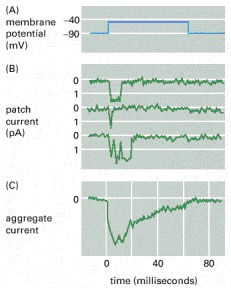
\includegraphics[width=.65\textwidth]{fig/ch11f32.jpg}
		\caption{Patch-clamp measurements for a single voltage-gated $Na^+$ channel 
			(Fig.~11.32 in~\cite{MolecularBiology:2002}). Notice that due to the low current intensity, the measurement method comprises integration that "smears" line shape. Also notice that the shape of the aggregate current comprises
different time contributions due to the different distances
of channels from the measurement tip.
			 \label{fig:Single_VoltageGatedChannel}}
\end{figure*}

As Fig.~\ref{fig:Single_VoltageGatedChannel} depicts,
an ion channel is open roughly for~$10^{-2}\ s$~and the 
peak amplitude is~$1.6*10^{-12}\ A$, so the maximum charge
that can be transferred in a single shot is~$1.6*10^{-14}\ Cb$,
which assumes~$10^5$~ions per shot per channel. 
(If we assume that the ions
pass the ion channel one by one, without pausing, the passage time of an ion is
\SI{0.1}{\milli\second}.
%is $10^{-7}\ s$.
Given that the electrolyte electrodes contribute 
a considerable delay, the value might be not accurate.)



The entered ions cannot leave sufficiently quickly 
the proximity of the channel's exit, so their potential prevents
the rest of ions from entering the membrane: the ion layer closes the channel.
Recall that the 
number of the uncompensated ions is about~$5*10^7$, the several
(typically several hundreds) simultanously working ion channels overcompensate the ion balance:
despite the forceful external potential, no more ions can enter
the membrane (the 'downhill' gradient cancels; if we use the approximation that the ions traverse the channel length instantly).
In the rest of the shown period, despite that the external voltage
(the square wave) is still present, the potential of the stalled ions
(the internal voltage) keeps the channel closed: no new rising edge (voltage gradient) arrives.
In the figure, the aggregate current enables us to estimate the 
total number of channels to be~$100-120$. 
Clearly, the aggregate current shows two effects: the individual ion channels' contributions, which are measured within the channels, have steep rising and falling edges. As the figure depicts, after~$20\ ms$~no more new openings happen.
Following that, the currents flow toward the point where
the aggregated current measured:
the charge on the membrane quietly discharges. 
(The reason of the decay is the same as in the case of
the \gls{AP}
a slow current flows on the surface; so their time constant is the same, althought the fluctuation due to the arrival time of the contributions
of the individual channels is more observable.)    Again, the external voltage
is stable, the internal voltage decreases, so the aggregate current decreases. The membrane's conductance does not change. However,
the resulting potential that directs the current is the sum of
the external and internal potentials. As the charge diffuses toward
the bulk region, the internal potential decays, and so does the measurable
aggregate current. 


Although the individual
ion channels open and close 'randomly', the repulsion force
on the two surfaces of the membrane acts as an additional valve; its discussion see in section~\ref{sec:Physics-ResourcesIonChannels}.
As \cite{MolecularBiology:2002} discusses,
'this potential difference ... exists across a plasma membrane only about $5\ nm$ thick,
so that the resulting voltage gradient is about $100,000\ V/cm$'.
\index{voltage gradient}
In a statistical sense, part of the ion channels can be open
after the population members received the 'open' signal, part of the population can be closed
or inactivated,
but when the layer enables, the ions in the proximal layer
can escape to the other side of the membrane.



It is also known that  for their adequate operation, the ion channels need to implement
three states: in addition to the 'on' and 'off' states, they can also be in an inactivated
state~\cite{ThreeStateUnidirectional:2004, MarkovianIonChannel:2005}.
However, the population of the ion channels has only 'on' and 'off' states;
furthermore, for some reason the population get "fatigued":
"the probability, that any individual channel
will be in the open state, decreases with time"~\cite{MolecularBiology:2002}. 
It is due to the finite resources, as we quantitatively discuss it in section~\ref{sec:Physics-ResourcesIonChannels}.

%\cite{HilleIonChannels:1999}

As Fig.~\ref{fig:Single_VoltageGatedChannel} depicts, it is the gradient (the rising edge), 
instead of the membrane potential, which 
starts the individual patch currents (and, of course, 
the aggregate current).
Depending on the environment of the channel's exit (the fluctuation
of the charge density), the channel has an a maximum 'let-in' time.
The representative patch currents show that the channel can definitely 
and quickly open, 


\subsubsection{Ion layers\label{sec:Physics-IonLayers}}

Semipermeable membranes, with ion channels in their walls, separating electrolyte segments with ion concentrations differing by orders of magnitude,  play a unique role in neuronal electric operation.
It is at least problematic to interpret the operation of the individual channels without understanding their dynamic
interaction with the other channels, the electrolyte, and the semipermeable membrane. 

We consider the external concentration constant: the extracellular
space is infinitely large, and the amount of ions remains by orders
of magnitude higher than the internal one. Our assumption is valid for the \textit{global static} concentration (we call it 'bulk'), but not for the \textit{local dynamic} one.
The voltage-controlled ion channels open when
on the lower concentration side, the local voltage exceeds some threshold value.

In the \textit{resting state} (without a voltage offset around the ion channels), the channels keep balance between the separated segments. 
However, when an ion channel gets open (meaning that ions from the high-concentration side can
pass through it to the low-concentration side), for a short period,
the ions change the \textit{local} concentration and potential of the electrolyte in the
proximity of the entrance and exit of the channels,
forming \hypertarget{membrane_layers}{two proximal layers}. 
The case drastically changes if an additional potential gradient appears.
In that case, (part of) the ion layer, formed on the
membrane's surface due to the charge arriving through the ion
channels, is  continuously removed by the macroscopic ion current from the immediate
proximity of the ion channels. The layer gets saturated later, and
the conditions of transferring ions
through the channels persist for longer, so they remain open, enabling a continuous
ion inflow (a macroscopic current; see the
discussion about  \hyperlink{voltage-clamping}{clamping dynamic operation} using  
\gls{AIS}).

The ion channels have three states, but their population has only two.
\index{ion channel!state}
Fundamentally, the lack or presence of \textit{unbalanced} ions in the proximal layers defines the 'open' and 'closed' states of the channel population. The individual
ion channels open and close in a stochastic way. In a statistical sense, part of the ion channels can be open, and another part can be closed or inactivated.
However, only when the layer's potential enables, can the ions in the proximal layer
escape to the other side of the membrane, even if the channel is open. 
The ion channels have no reason to re-open because of the lack of offset voltage (and that layer).
That is, primarily, the presence of the layers on the two sides of the membrane defines the ion inflow,
and the individual ion channels  can freely (re)open, close, or inactivate
until the layer provides a sufficiently large potential offset.
This transient state is the key to understanding the dynamic operation of neurons.

There is a strong electric field on the boundary of the segments. 
As \cite{MolecularBiology:2002} discusses,
'an electrical potential difference about 50–100 mV ... exists across a plasma membrane only about $5\ nm$ thick,
 so the resulting voltage gradient is about $100,000\ V/cm$'.
\index{voltage gradient}
In their 'off' state, the voltage-controlled ion channels are mechanically closed, so the ions cannot follow that gradient.  
However, when (due to the collected synaptic charge or the significant slope of the arriving spike~\cite{LosonczyIntegrative:2006} or clamping) a voltage offset appears at the  ion channel, so it opens. Due to the enormous gradient, ions rush in
from the extracellular segment into the intracellular one. This means a high speed, that is, a 'fast' current, see Eq.~(\ref{eq:StokesCurrent}).

However, upon arriving at the other side of the  membrane, they experience the
electric field disappearing, so the stream of ions stalls. The stalled ions 
increase the local potential (see section~\ref{Physics-OscillatorDifferentiator}) around the  channel's exit,
and the ions will move along the parallel potential gradient toward neighboring 
channel exits. 
'The description just given of an action potential concerns only a small patch of plasma membrane.
However, the self-amplifying depolarization of the patch, 
is sufficient to depolarize neighboring regions of the membrane,
which then go through the same cycle. In this way,
the action potential spreads as a traveling wave from the initial site of depolarization
to involve the entire plasma membrane' \cite{MolecularBiology:2002}.
The depolarization happens in an avalanche-like way \cite{NeuronalAvalanches:2003} over the entire membrane surface.  
This process creates ion-rich layers in the proximity of the membrane
on both sides. At the end of the process, the potential in the layer on the intracellular side temporarily reaches
the  potential inside the bulk of the extracellular side.
\index{layer!potential}
The ions in the layer experience two forces: in the direction 
parallel to the membrane's surface, the electric repulsion due to the fellow ions in the same layer; furthermore, in the perpendicular direction, the attraction of the ions
in the opposite layer.

The first force acts in distributing the potential uniformly  over the surface, and \textit{in this way (per definitionem), an ion 
current flows in parallel with the surface}. This ion current is slow: the ions are moving 
in a viscous solution under the effect of a potential gradient (see Eq.~(\ref{eq:StokesCurrent})), if any. In the lack of external potential, it is of type relaxation. The presence of a current drain (such as \gls{AIS}
on the membrane or the axonal arbor on the axon) also means a potential difference,  and an exponential discharge function of type $exp(-\beta *t)$ 
describes that current, $\beta$ is a time constant.

The second one acts against diffusion and prevents the ions from leaving the layer.
\index{layer!diffusion}
Until that current stops (due to the saturation of the layer),
\textit{an ion current will flow in the direction perpendicular to the surface}.
\index{layer!current}
That current is "fast" only within the ion channel until the driving force disappears,
and becomes "slow" in the electrolyte layer, where the received charge saturates the layer. A current of form $(1-exp(-\alpha *t))$ can describe the saturation, where $\alpha$ is a time constant.
 Recall that the current's speed
depends on the voltage gradient, so the intensity and the temporal behavior of the 
currents are different, even between the "parallel" and "perpendicular" current directions, given that two different mechanisms control the process,
\index{voltage gradient}
despite that we consider the motion of the same charged particles. As a result of the two processes, a function of type $(1-exp(-\alpha *t))*exp(-\beta *t)$ describe the local charge distribution in the function of time. Although the timing constants change
as the potential changes, we use the approximation that
the layer is thin; furthermore, its concentration and potential have zero gradients in a direction perpendicular to the membrane. However,
a steep potential gradient exists between the layer
and the rest of the segment.
\index{layer!thickness}



The 'caps' on the top of the ion channels act as
individual regulators, and the ion channels continuously and randomly open, close, and inactivate. Their statistical population enables a
macroscopic ion inflow throughout the surface and the electric repulsion distributes
the charge over the surface, tending to make the local potential uniform over the surface.
The repulsion and attraction forces
on the two surfaces of the membrane around the channel's exit act as an additional valve on the ion transport:
the population 
of ion channels must cooperate with them, given that the ions move 'downhill'.


This behavior explains why ion currents across the membrane
start up with a sharp exponential rise~\cite{SodiumCurrentDelay:2006}
(one of the big mistakes was fitting polynomial lines~\cite{HodgkinHuxley:1952}
to those critical regions, comprising both exponential and no-current regions: it hides the sudden change of membrane's current~\cite{SodiumCurrentDelay:2006}
caused by the state change of the ion channels); why initiating an
\gls{AP} has precise timings (both the charge-up signal and pressing
ions through the \gls{AIS});
why axonal arbors can provide a precise
``Begin Computing'' signal. 
Measuring the conductance of ion channels, requires special care.
As discussed in section~\ref{sec:PHYSICS_MEASURINGCONDUCTANCE}, it is easy to
make a systematic error, given that the measurement method can affect the result. 


We posit explicitly that our parameters can be directly concluded from the measurable parameters such as membrane surface size, its ion channel density, specific membrane capacitance and absolute resistance of the \gls{AIS}.
Having those parameters of components of the non-living matter, plus the time course of the input currents,
we can describe how and why a the living matter shows the behavior we can observe.
This exact discussion provides an excellent base for understanding neuronal assemblies' operation,
furthermore revealing details of neuronal information storage and transfer.


This behavior explains why ion currents
start up with a sharp exponential rise \cite{SodiumCurrentDelay:2006}
(fitting polynomial lines \cite{HodgkinHuxley:1952}
to those critical regions was a big mistake: it hides the sudden change
caused by the state change (opening) of the ion channels, and that
the 'rising edge' is actually described by an exponential increase); why initiating an \gls{AP} 
has precise timings (both the charge-up signal and pressing
ions through the \gls{AIS}); why axonal arbors can pr
ovide a precise
`ComputingBegin' signal. For the details, see the following subsections.
\hyperlink{electric_conductance}
{Measuring the conductance}
of ion channels, requires special care.
\index{conductance}
It is easy to make a systematic error, given that the measurement device can affect the result.

Notice that the charged layers mean that a population
of ion channels must cooperate. Although the individual
\index{layer!ion channels}
\index{ion channel!operation}
ion channels open and close 'randomly', the repulsion force
on the two surfaces of the membrane acts as an additional valve. In a statistical sense, some ion channels are open
after the population members received the 'open' signal,
but when they are open, only the ions in the proximal layer
can escape to the other side of the membrane.


%\subsection{Role of proteins\label{sec:Single-RoleOfProteins}}

"When measuring currents through small membrane segments, the conductance events appear in a quantized steps,
i.e. one observes a switching between current-on and currentoff events. In biological membranes one normally assumes
that this phenomenon is caused by the opening and closing
of ion channel proteins (Fig. 3a). The two conduction states
are called open and closed channels. As already described
above, these channel proteins play an important role in the
Hodgkin-Huxley model of nerve pulse conduction. Interestingly, one finds very similar events in synthetic membranes
that are free of proteins (e.g., [10, 11]), in particular if one
is close to the melting transition (Fig. 3b). Both current
amplitude and the typical opening time scales are practically indistinguishable from those of protein-containing
membranes. Obviously, the finding of quantized current
events is not a proof for the activity of proteins even though
this is what is generally assumed since membranes close
to transition display the same characteristics. Whether the
events in protein-containing membranes and those in pure
lipid membranes have the same origin is yet an open question."~\cite{HeimburgPhysikOfNerves:2009}

